\section{Problem 1}

\subsection*{Step 1: Acceleration Phase (0 to $t_1$)}

- Initial velocity, $v_0 = 0 \text{ m/s}$ \\
- Final velocity at $t_1$, $v_1 = 4 \text{ m/s}$ \\
- Time interval, $t_1 = 4 \text{ s}$

The acceleration $a_1$ is calculated as:
\[
a_1 = \frac{v_1 - v_0}{t_1 - 0} = \frac{4 - 0}{4} = 1 \text{ m/s}^2
\]

The displacement during this phase $x_1$ is:
\[
x_1 = \frac{1}{2} a_1 t_1^2 = \frac{1}{2} \times 1 \times 4^2 = 8 \text{ m}
\]

\subsection*{Step 2: Constant Velocity Phase ($t_1$ to $t_2$)}

- Velocity $v = 4 \text{ m/s}$ \\
- Time interval $t_2 - t_1 = 10 - 4 = 6 \text{ s}$ \\
The displacement during this phase $x_2$ is:
\[
x_2 = v \cdot (t_2 - t_1) = 4 \times 6 = 24 \text{ m}
\]

\subsection*{Step 3: Deceleration Phase ($t_2$ to $t_3$)}

- Initial velocity $v_2 = 4 \text{ m/s}$ \\
- Final velocity $v_3 = 0 \text{ m/s}$ \\
- Time interval $t_3 - t_2 = 18 - 10 = 8 \text{ s}$ \\
The deceleration $a_3$ is:
\[
a_3 = \frac{v_3 - v_2}{t_3 - t_2} = \frac{0 - 4}{8} = -0.5 \text{ m/s}^2
\] \\
The displacement during this phase $x_3$ is:
\[
x_3 = v_2 \cdot (t_3 - t_2) + \frac{1}{2} a_3 (t_3 - t_2)^2 = 4 \times 8 + \frac{1}{2} \times (-0.5) \times 8^2 = 16 \text{ m}
\]

\subsection*{Step 4: Total Displacement and Average Velocity}

The total displacement from $t_1$ to $t_3$ is:
\[
\text{Total Displacement} = x_2 + x_3 = 24 + 16 = 40 \text{ m}
\]

The average velocity over the interval $[t_1, t_3]$ is:
\[
v_{\text{avg}} = \frac{\text{Total Displacement}}{t_3 - t_1} = \frac{40}{18 - 4} = \frac{40}{14} \approx 2.86 \text{ m/s}
\]

\subsection*{Final Answer}

- \textbf{Total displacement from $t_1$ to $t_3$: 40 meters}
- \textbf{Average velocity over the time interval $[t_1, t_3]$: 2.86 m/s}

\subsection*{Plots}
Below are the plots for acceleration and displacement as functions of time:

\begin{figure}[h]
\centering
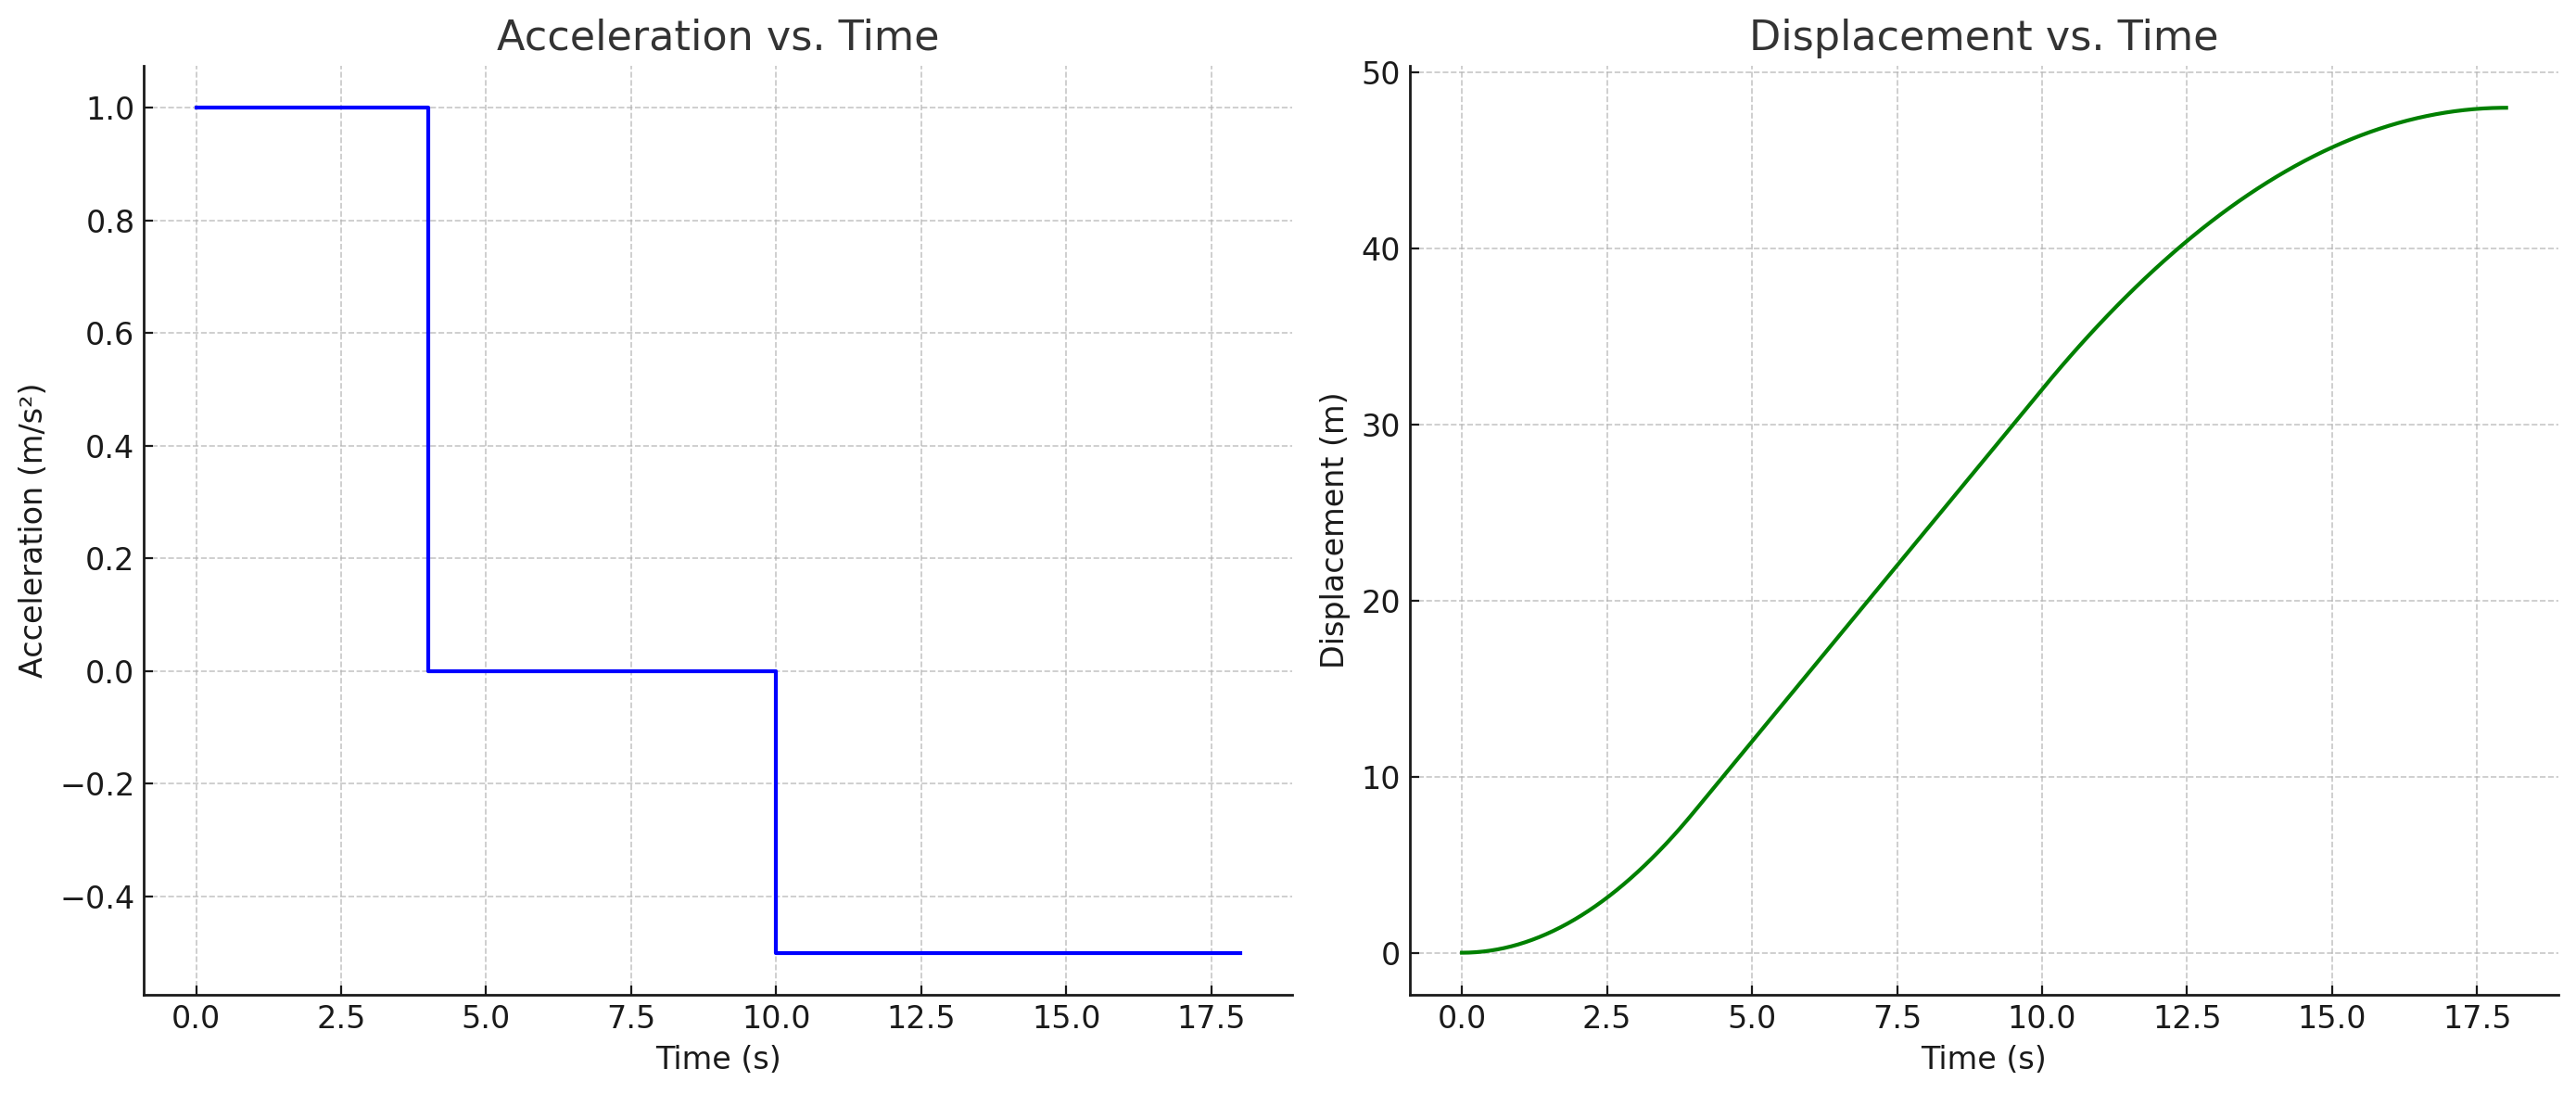
\includegraphics[width=0.8\textwidth]{acceleration_displacement.png}
\caption{Acceleration and Displacement vs. Time}
\end{figure}
